\documentclass[12pt, a4paper]{article}
\usepackage [ngerman]{babel}
\usepackage[utf8]{inputenc}
\usepackage[T1]{fontenc}
%\renewcommand{\rmdefault}{phv} % Arial
%\renewcommand{\sfdefault}{phv} % Arial
\usepackage{color}
\usepackage{fancyhdr}
\usepackage{graphicx}
\usepackage{geometry}

\parindent0em

%Inhaltsverzeichnis mit Links füllen
\usepackage{hyperref}
\hypersetup{
    colorlinks,
    citecolor=black,
    filecolor=black,
    linkcolor=black,
    urlcolor=black
}

\geometry{verbose,a4paper,bmargin=30mm,lmargin=25mm,rmargin=20mm}

\pagestyle{fancy} %eigener Seitenstil
\fancyhf{} %alle Kopf- und Fußzeilenfelder bereinigen
\fancyhead[L]{Programmieren 3} %Kopfzeile links
\fancyhead[C]{Robin Hake \\ Benedikt Brüntrup} %zentrierte Kopfzeile
\fancyhead[R]{
\includegraphics[width=4cm]{Bilder/HS_OWL_RGB_Rot.jpg}} %Kopfzeile rechts
\renewcommand{\headrulewidth}{0.4pt} %obere Trennlinie
\fancyfoot[C]{\thepage} %Seitennummer
\renewcommand{\footrulewidth}{0.4pt} %untere Trennlinie


\begin{document}
\begin{titlepage}
Hochschule Ostwestfalen-Lippe \\
Fachbereich 8 - Umweltingeneurwesen und Angewandte Informatik \\
Fachgebiet Angewandte Informatik \\
Programmieren 3 \\
5. Semester WS 2015/16\\
\vspace{2cm}

\begin{center}
\begin{Large}
\textbf{Dokumentation} \\
\end{Large}
\vspace{2cm}

\begin{Large}
\textbf {Implementierung eines Prototypen für eine Verwaltungssoftware für ein Call-Center} \\[0.35cm]
\end{Large}
Von \\[0.35cm]
Robin Hake \\
15306070 \\[0.35cm]
und\\[0.35cm]
Benedikt Brüntrup \\
15306067 \\[0.35cm]
\end{center}

\vfill
Erstprüfer: Prof. Dr. Ralf Hesse \\
Eingereicht am: {\today}
\end{titlepage}

\newpage
\tableofcontents


\vfill
\newpage


\section{Aufgabenstellung}
Als Abschlussarbeit des Moduls \glqq Programmiersprachen 3\grqq{} sieht die Prüfungsordnung die Abgabe eines in JavaEE implementierten Software-Projekts vor. Hierzu ist von den Professor Ralf Hesse eine Liste mit möglichen Abschlussthemen bereitgestellt worden. Von dieser Liste sollte sich ein Thema ausgesucht werden und zwei Anwendungsszenarien des Themas in einen Software-Prototyp umgesetzt werden. Der Software-Prototyp ist dabei auf Basis eines dreischichtigen Ansatz umzusetzen.  Die Gruppe Robin Hake und Benedikt Brüntrup entschloss sich das Thema \glqq Verwaltungssoftware für ein Call-Center\grqq{} umzusetzen.

\section{Projektplanung}
Zu Beginn der Projektplanung wurde mit Hilfe eines Use-Case-Diagramms ermittelt was das Projekt alles können soll. Die Ermittlungen haben ergeben, dass es einen Administrator und Standardbenutzer geben soll. Der Administrator soll Benutzer verwalten können und die Standardbenutzer sollen mit Tickets arbeiten können. Genauere Details zur Anforderungsanalyse kann den Use-Case-Diagramm der \textit{Abbildung 1} entnommen werden.

\begin{figure}[h]
	\begin{center}
	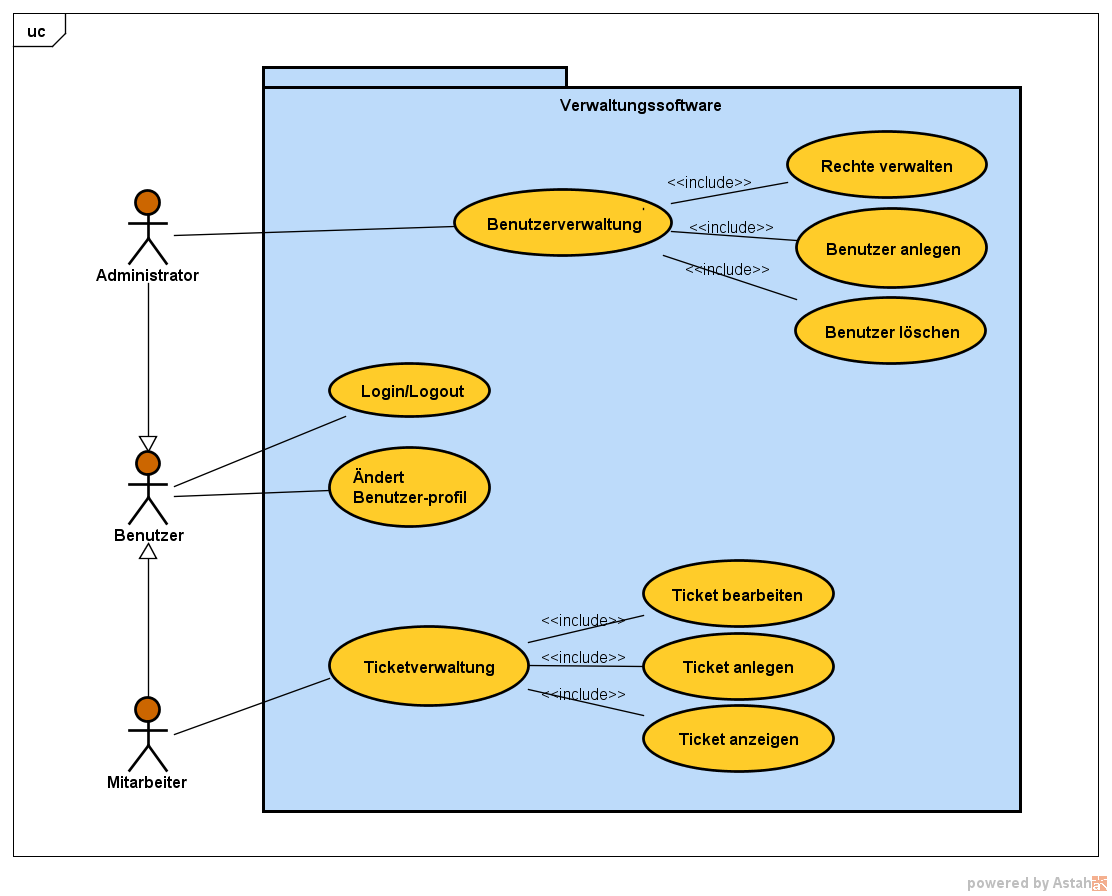
\includegraphics[width=120mm]{Bilder/UseCaseAnforderungsanalyse.png}
	\end{center}
	\caption{Anforderungsanalyse als Use-Case-Diagramm}
\end{figure}


Als nächstes wurde mit PowerPoint ein erster Designentwurf für die Weboberfläche des Projektes entworfen. Hierbei wurde sich für ein fensterbasiertes Design entschlossen. Dieses bietet den Vorteil, dass das Projekt einfach erweitert werden kann. Soll das Software-Produkt eine neue Funktion haben kann einfach ein neues Fenster hinzugefügt werden. Die folgende Abbildung zeigt den ersten Designentwurf mit PowerPoint.

\section{Literaturverzeichnis}

\subsection*{Literatur}

\textsc{Felinto, D. $ \& $ Pan, M} (2013): \textit{Game Development with Blender} - Cengage Delmar
\\
\subsection*{Onlinequellen}
\begin{itemize}
	\item \url{http://www.blenderhilfe.de}
	\item \url{http://www.blender.org}
	\item \url{https://de.wikibooks.org/wiki/Blender_Dokumentation}
\end{itemize}

\end{document}